%\documentclass[twoside,twocolumn,spanish]{article}
\documentclass{article}
\usepackage[T1]{fontenc}
\usepackage[utf8]{inputenc}
\usepackage{graphicx}
\usepackage[spanish]{babel}
\usepackage{amssymb,amsmath,geometry,multicol,spalign,hyperref}
\setlength\columnsep{20pt}
\usepackage[usenames,dvipsnames]{xcolor}
\usepackage{tikz,mathtools}
\usepackage{pgfplots}
\pgfplotsset{width=5cm,compat=1.12}
\usepgfplotslibrary{fillbetween}

\title{Cálculo de la aceleración de la gravedad mediante un péndulo físico}
\author{Andoni Latorre Galarraga \\ \href{mailto:alatorre73@alumno.uned.es}{alatorre73@alumno.uned.es}}
\date{}
\begin{document}

\maketitle
\begin{abstract}
Se estudia la relacíon entre el periodo de oscilación de un péndulo físico y la distancia entre el eje de rotación y el centro de masas de dicho péndulo. A partir de los datos experimentales se calcula el valor de la aceleración de la gravedad $g$.
\end{abstract}

\begin{multicols}{2}

\section{Fundamento Teórico}
Si se tiene un cuerpo rígido, de masa $M$, suspendido en un eje de giro $O$ a una distancia $b$ del centro de masas del objeto, $C$. Cuando el objeto está desplazado de su posición de equilibrio por un ángulo $\theta$. La aceleración tangencial del centro de masas se puede expresar de dos formas distintas, al igualar estas se tiene.
$$
-M g b \sen(\theta) = I \frac{d^2 \theta}{dt^2}
$$
Donde $I$ es el momento de inercia del cuerpo respecto al eje $O$.\\
Cuando se tienen valores pequeños de $\theta$ , menores a $20^\circ$, se puede aproximar $\theta \sim \sen(\theta)$.
$$
-M g b \theta = I \frac{d^2 \theta}{dt^2}
$$
Que tiene por solución $\sen \left( \theta \sqrt{\frac{Mgb}{I}} + \phi \right) + C$. Que corresponde a un movimiento armónico simple de periodoP
$$
T = 2\pi \sqrt{\frac{I}{Mgb}}
$$
Si se llama $I_0$ al momento de inercia respecto al eje paralelo a $O$ que pasa por $C$, por el teorema de Huygens-Steiner, se tiene:
$$
T = 2\pi \sqrt{\frac{I_0 + Mb^2}{Mgb}}
$$
$I_0$ está relacionado con er radio de giro, $k$, mediante la relación $k = \sqrt{\frac{I_0}{M}}$. Por lo tanto,
$$
T = 2\pi \sqrt{\frac{Mk^2 + Mb^2}{Mgb}} = 2\pi \sqrt{\frac{k^2 + b^2}{gb}}
$$
Utilizaremos esta última expresión para el periodo de oscilación, en nuestro cálculo de $g$. Linealizamos la expresión de la siguiente manera:
$$
\textcolor{blue}{bT^2} = 4\pi^2 \frac{k^2}{g} + 4\pi^2 \frac{\textcolor{blue}{b^2}}{g}
$$
Obtenemos una relación lineal entre $bT^2$ y $b^2$. Estimaremos la pendiente y la ordenada en el origen de dicha relación para obtener el valor de $g$.

\section{Dispositivo Experimental}
En nuestro experimento hemos utilizado una varilla metálica como péndulo. La varilla tine unas marcas cada centímetro. Al dadas estas marcas, supondremos que no hay error en $b$. Estas marcas son tales que se puede situar un pequeño trozo de metal mediante un tornillo de presión para sujetar la varilla y que esta tenga como eje de rotación la marca en la que se situa el metal triangular. Ademas, la varilla central indica el centro de masas. De esta manera, contando ranunas desde el centro de la varilla podemos conocer el valor de $b$. En la Fig. 1 se puede ver el dispositivo experimental ya montado.
\begin{center}
    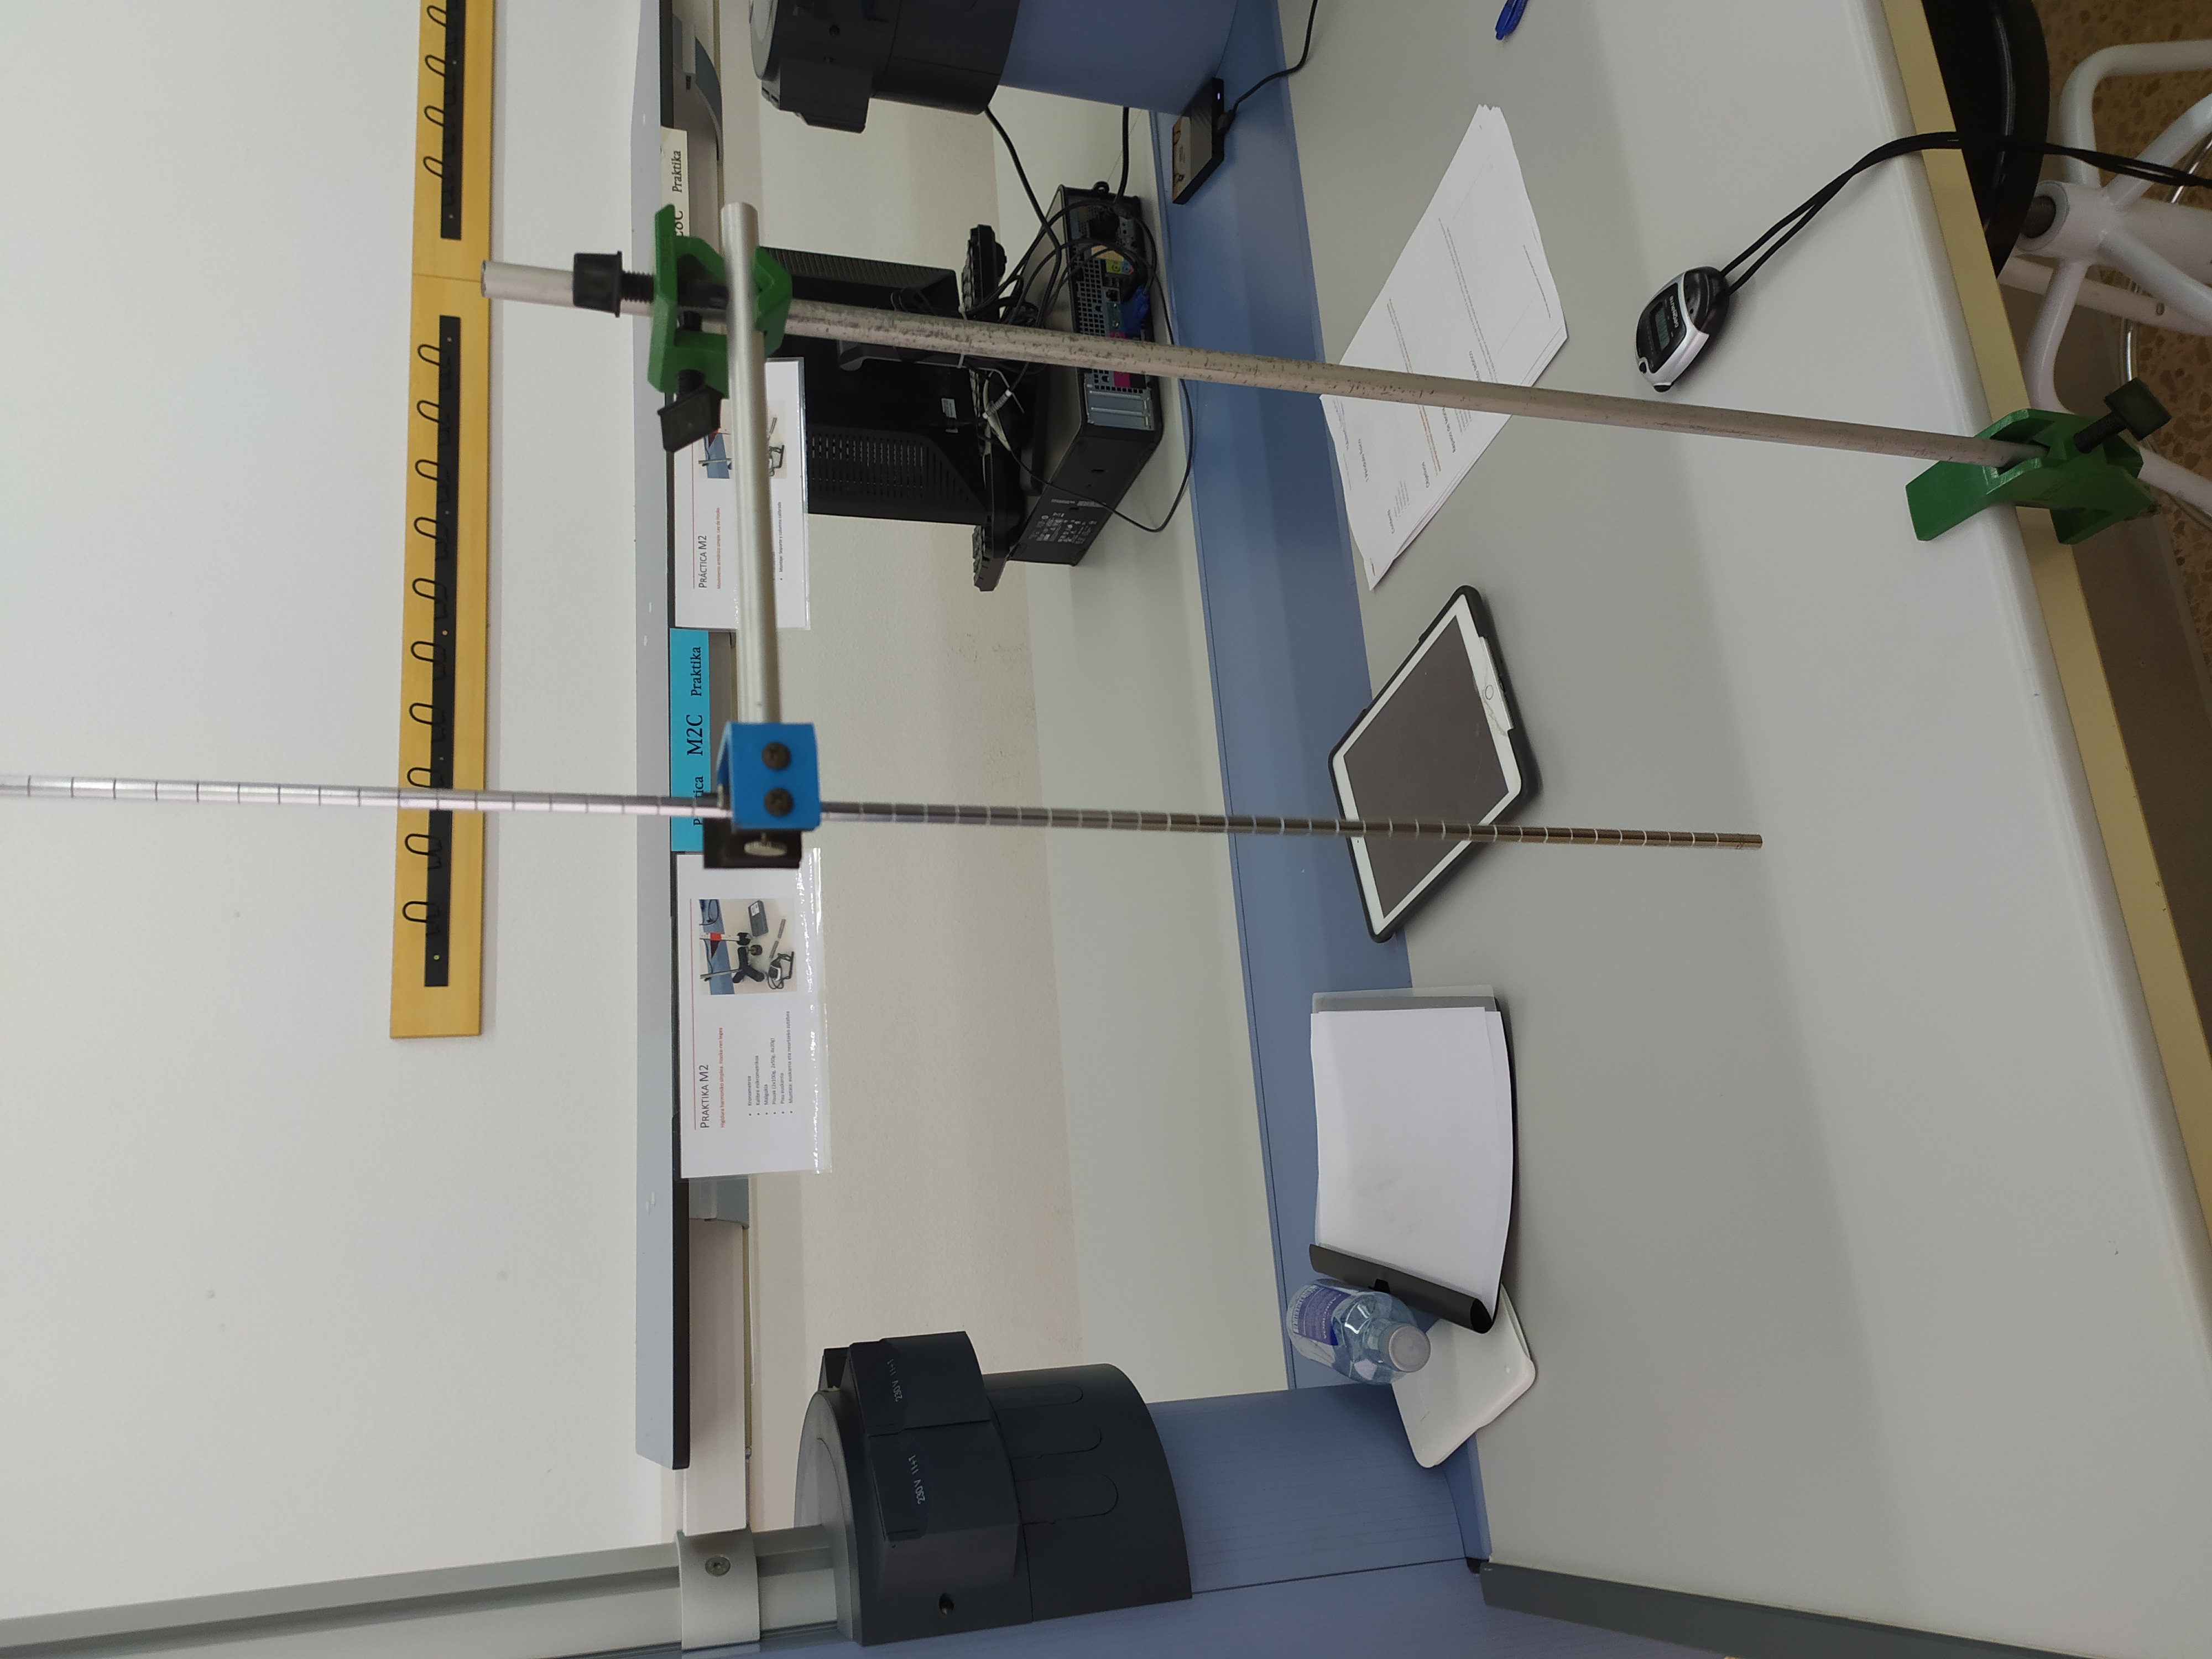
\includegraphics[scale=0.06, angle=-90]{figures/c2.png}\\
    Figura 1: Dispositivo experimental montado.
\end{center}

\section{Procedimiento y Resultados}
Hemos tomado mediciones para $b\in \{6\text{cm}, 7\text{cm}, \cdots, 30\text{cm}, 31\text{cm}\}$. Para cada valor de $b$ hemos tomado 5 tiempos independientes, cada uno de estos correspondiente a 10 oscilaciones (excepto para $23 \text{cm}\le b \le 26\text{cm}$ que hemos tomado 20). Siempre hemos tenído cudado de que la varilla no oscile con ángulos superiores a $20^\circ$. Los datos obtenidos son los siguientes:
$$
    \begin{array}{|c||c|c|c|c|c|} \hline
        b\text{(m)} & T_1\text{(s)} & T_2\text{(s)} & T_3\text{(s)} & T_4\text{(s)} & T_5\text{(s)} \\ \hline\hline
        0.08 & 15.07 & 15.13 & 15.19 & 15.13 & 15.00  \\ \hline
        0.09 & 14.31 & 13.28 & 14.31 & 14.28 & 14.38  \\ \hline
        0.10 & 13.91 & 13.91 & 13.97 & 13.82 & 13.78  \\ \hline
        0.11 & 13.53 & 13.44 & 13.25 & 13.37 & 13.78  \\ \hline
        0.12 & 13.25 & 13.37 & 13.40 & 13.16 & 13.19  \\ \hline
        0.13 & 13.06 & 12.97 & 13.03 & 13.12 & 12.97  \\ \hline
        0.14 & 12.84 & 12.81 & 12.88 & 12.84 & 12.72  \\ \hline
        0.15 & 12.56 & 12.50 & 12.72 & 12.69 & 12.78  \\ \hline
        0.16 & 12.53 & 12.63 & 12.59 & 12.50 & 12.47  \\ \hline
        0.17 & 12.44 & 12.41 & 12.53 & 12.44 & 12.50  \\ \hline
        0.18 & 12.44 & 12.43 & 12.50 & 12.54 & 12.47  \\ \hline
        0.19 & 12.34 & 12.47 & 12.31 & 12.35 & 12.28  \\ \hline
        0.20 & 12.37 & 12.50 & 12.37 & 12.47 & 12.43  \\ \hline
        0.21 & 12.16 & 12.40 & 12.56 & 12.60 & 12.19  \\ \hline
        0.22 & 12.46 & 12.53 & 12.62 & 12.53 & 12.37  \\ \hline
        0.23 & 12.59 & 12.50 & 12.41 & 12.62 & 12.56  \\ \hline
        0.24 & 12.56 & 12.62 & 12.57 & 12.59 & 12.59  \\ \hline
        0.25 & 25.03 & 25.22 & 25.31 & 25.18 & 25.35  \\ \hline
        0.26 & 25.34 & 25.37 & 25.41 & 25.44 & 25.25  \\ \hline
        0.27 & 25.50 & 25.47 & 25.59 & 25.57 & 25.60  \\ \hline
        0.28 & 25.78 & 24.38 & 25.78 & 25.72 & 25.59  \\ \hline
        0.29 & 12.97 & 12.94 & 13.03 & 13.00 & 13.00  \\ \hline
        0.30 & 13.00 & 13.06 & 12.91 & 13.03 & 13.07  \\ \hline
        0.31 & 12.94 & 13.12 & 13.19 & 13.13 & 13.16  \\ \hline
        0.32 & 13.29 & 13.22 & 13.35 & 13.09 & 13.19  \\ \hline
        0.33 & 13.50 & 13.54 & 13.21 & 13.41 & 13.22  \\ \hline
    \end{array}
$$
Tomaremos como valor esperado del tiempo, $T^*$, la media aritmetica de los 5 tiempos (divididos entre 10 o 20 segun corresponda). Para estimar el error absoluto, $\epsilon_{T^*}$, el error estándard de la media como se indica en \cite{manual} p. 48.
$$
T^* = \frac{1}{5} \sum_{i=1}^5 \frac{T_i}{10} \quad
\epsilon_{T^*} = \sqrt{\frac{1}{5^2} \sum_{i=1}^5 (\frac{T_i}{10} - T^*)^2}
$$
Los redondeos se han realizado como se indica en \cite{manual} p. 22. Primero se redondea $\epsilon$ a una cifra significativa (dos si la primera es 1). Despues, se redondea $T^*$ de manera que la última cifra significativa se del mismo orden decimal que $\epsilon$. Ahora, podemos calcular ${T^*}^2b$ y su error correspondiente con la ecuación 3.6 de \cite{manual}. Estos se redondean como antes. El error de ${T^*}^2b$ viene dado por:
$$
\epsilon_{{T^*}^2b} =
\sqrt{\left| \frac{d {T^*}^2b}{d T^*} \right|^2 \epsilon_{T^*}^2}=
2bT^* \epsilon_{T^*}
$$
$$
  \begin{array}{|l|l|l|l|l|} \hline
    b\text{(m)} & T^*\text{(s)} & \epsilon_{T^*}\text{(s)} & {T^*}^2b\text{(s\textsuperscript{2}m)} & \epsilon_{{T^*}^2b}\text{(s\textsuperscript{2}m)}\\ \hline \hline
    0.08 & 1.510 & 0.003 & 0.1824 & 0.0007  \\ \hline
    0.09 & 1.411 & 0.019 & 0.179 & 0.005  \\ \hline
    0.10 & 1.388 & 0.003 & 0.1927 & 0.0008  \\ \hline
    0.11 & 1.347 & 0.008 & 0.200 & 0.002  \\ \hline
    0.12 & 1.327 & 0.004 & 0.2113 & 0.0013  \\ \hline
    0.13 & 1.303 & 0.003 & 0.2207 & 0.0010  \\ \hline
    0.14 & 1.282 & 0.002 & 0.2301 & 0.0007  \\ \hline
    0.15 & 1.265 & 0.005 & 0.2400 & 0.0019  \\ \hline
    0.16 & 1.254 & 0.003 & 0.2516 & 0.0012  \\ \hline
    0.17 & 1.246 & 0.002 & 0.2639 & 0.0008  \\ \hline
    0.18 & 1.2476 & 0.0018 & 0.2802 & 0.0008  \\ \hline
    0.19 & 1.235 & 0.003 & 0.2898 & 0.0014  \\ \hline
    0.20 & 1.243 & 0.002 & 0.3090 & 0.0010  \\ \hline
    0.21 & 1.238 & 0.008 & 0.322 & 0.004  \\ \hline
    0.22 & 1.250 & 0.004 & 0.344 & 0.002  \\ \hline
    0.23 & 1.254 & 0.003 & 0.3617 & 0.0017  \\ \hline
    0.24 & 1.2586 & 0.0009 & 0.3802 & 0.0005  \\ \hline
    0.25 & 1.261 & 0.003 & 0.3975 & 0.0019  \\ \hline
    0.26 & 1.2681 & 0.0015 & 0.4181 & 0.0010  \\ \hline
    0.27 & 1.2773 & 0.0012 & 0.4405 & 0.0008  \\ \hline
    0.28 & 1.273 & 0.012 & 0.454 & 0.009  \\ \hline
    0.29 & 1.2988 & 0.0014 & 0.4892 & 0.0011  \\ \hline
    0.30 & 1.301 & 0.003 & 0.508 & 0.002  \\ \hline
    0.31 & 1.311 & 0.004 & 0.533 & 0.003  \\ \hline
    0.32 & 1.323 & 0.004 & 0.560 & 0.003  \\ \hline
    0.33 & 1.338 & 0.006 & 0.591 & 0.005  \\ \hline
    \end{array}
$$
Finálmente, se hace el cálculo de la regresión lineal y sus errores con las ecuaciones de \cite{manual} p. 79-80.
\begin{center}
\includegraphics[scale=0.7]{figures/regresión.png}
\end{center}
Se tiene que
$$
m = 4\frac{\pi^2}{g} = (3.98 \pm 0.02) \text{ s\textsuperscript{2}m\textsuperscript{-1}}
$$
$$
n = 4 \pi^2 \frac{k^2}{g} = (0.1508 \pm 0.0012) \text{ s\textsuperscript{2}m}
$$
Utilizando la ecuación 3.6 de \cite{manual} podemos calcular los errores de $g$ y $k$.
$$
\epsilon_g =
\sqrt{ \left| \frac{dg}{dm} \right|^2 \epsilon_m^2 } =
\sqrt{ \left| \frac{d \frac{4\pi^2}{m}}{dm} \right|^2 \epsilon_m^2 } =
\frac{4\pi^2}{m^2}\epsilon_m
$$
$$
\epsilon_k =
\sqrt{
  \left| \frac{\partial k}{\partial g} \right|^2 \epsilon_g^2 +
  \left| \frac{\partial k}{\partial n} \right|^2 \epsilon_n^2
}
$$
$$
\epsilon_k = \sqrt{
  \left| \frac{\partial \frac{\sqrt{ng}}{2\pi}}{\partial g} \right|^2 \epsilon_g^2 +
  \left| \frac{\partial \frac{\sqrt{ng}}{2\pi}}{\partial n} \right|^2 \epsilon_n^2
}
$$
$$
\epsilon_k = \sqrt{
  \left| \frac{n}{4\pi\sqrt{ng}} \right|^2 \epsilon_g^2 +
  \left| \frac{g}{4\pi\sqrt{ng}} \right|^2 \epsilon_n^2
}
$$
$$
\epsilon_k =
\frac{1}{\pi} \sqrt{\frac{n}{g} \epsilon_g^2 + \frac{g}{n} \epsilon_n^2}
$$
Obtenemos
$$
g = (9.92 \pm 0.05) \text{ ms\textsuperscript{-2}}
$$
$$
k = (0.195 \pm 0.004) \text{ m}
$$
\section{Conclusiones}

\begin{thebibliography}{1}

  \bibitem{manual}Manual de la asignatura. Versión 3.7

\end{thebibliography}

\end{multicols}

\end{document}
